\providecommand{\main}{../../../..}
\documentclass[\main/dresen_thesis.tex]{subfiles}

\begin{document}
  \begin{figure}[tb]
    \centering
    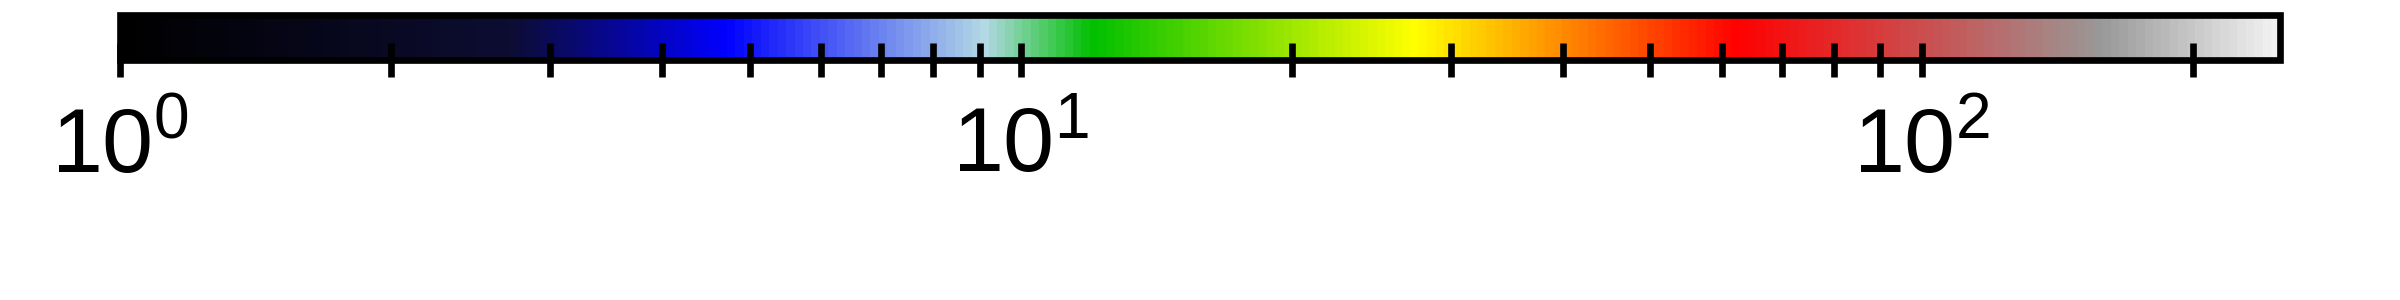
\includegraphics{monolayers_ML-Ac-CoFe-C_GISANS_SVcbar_parallelBeam}
    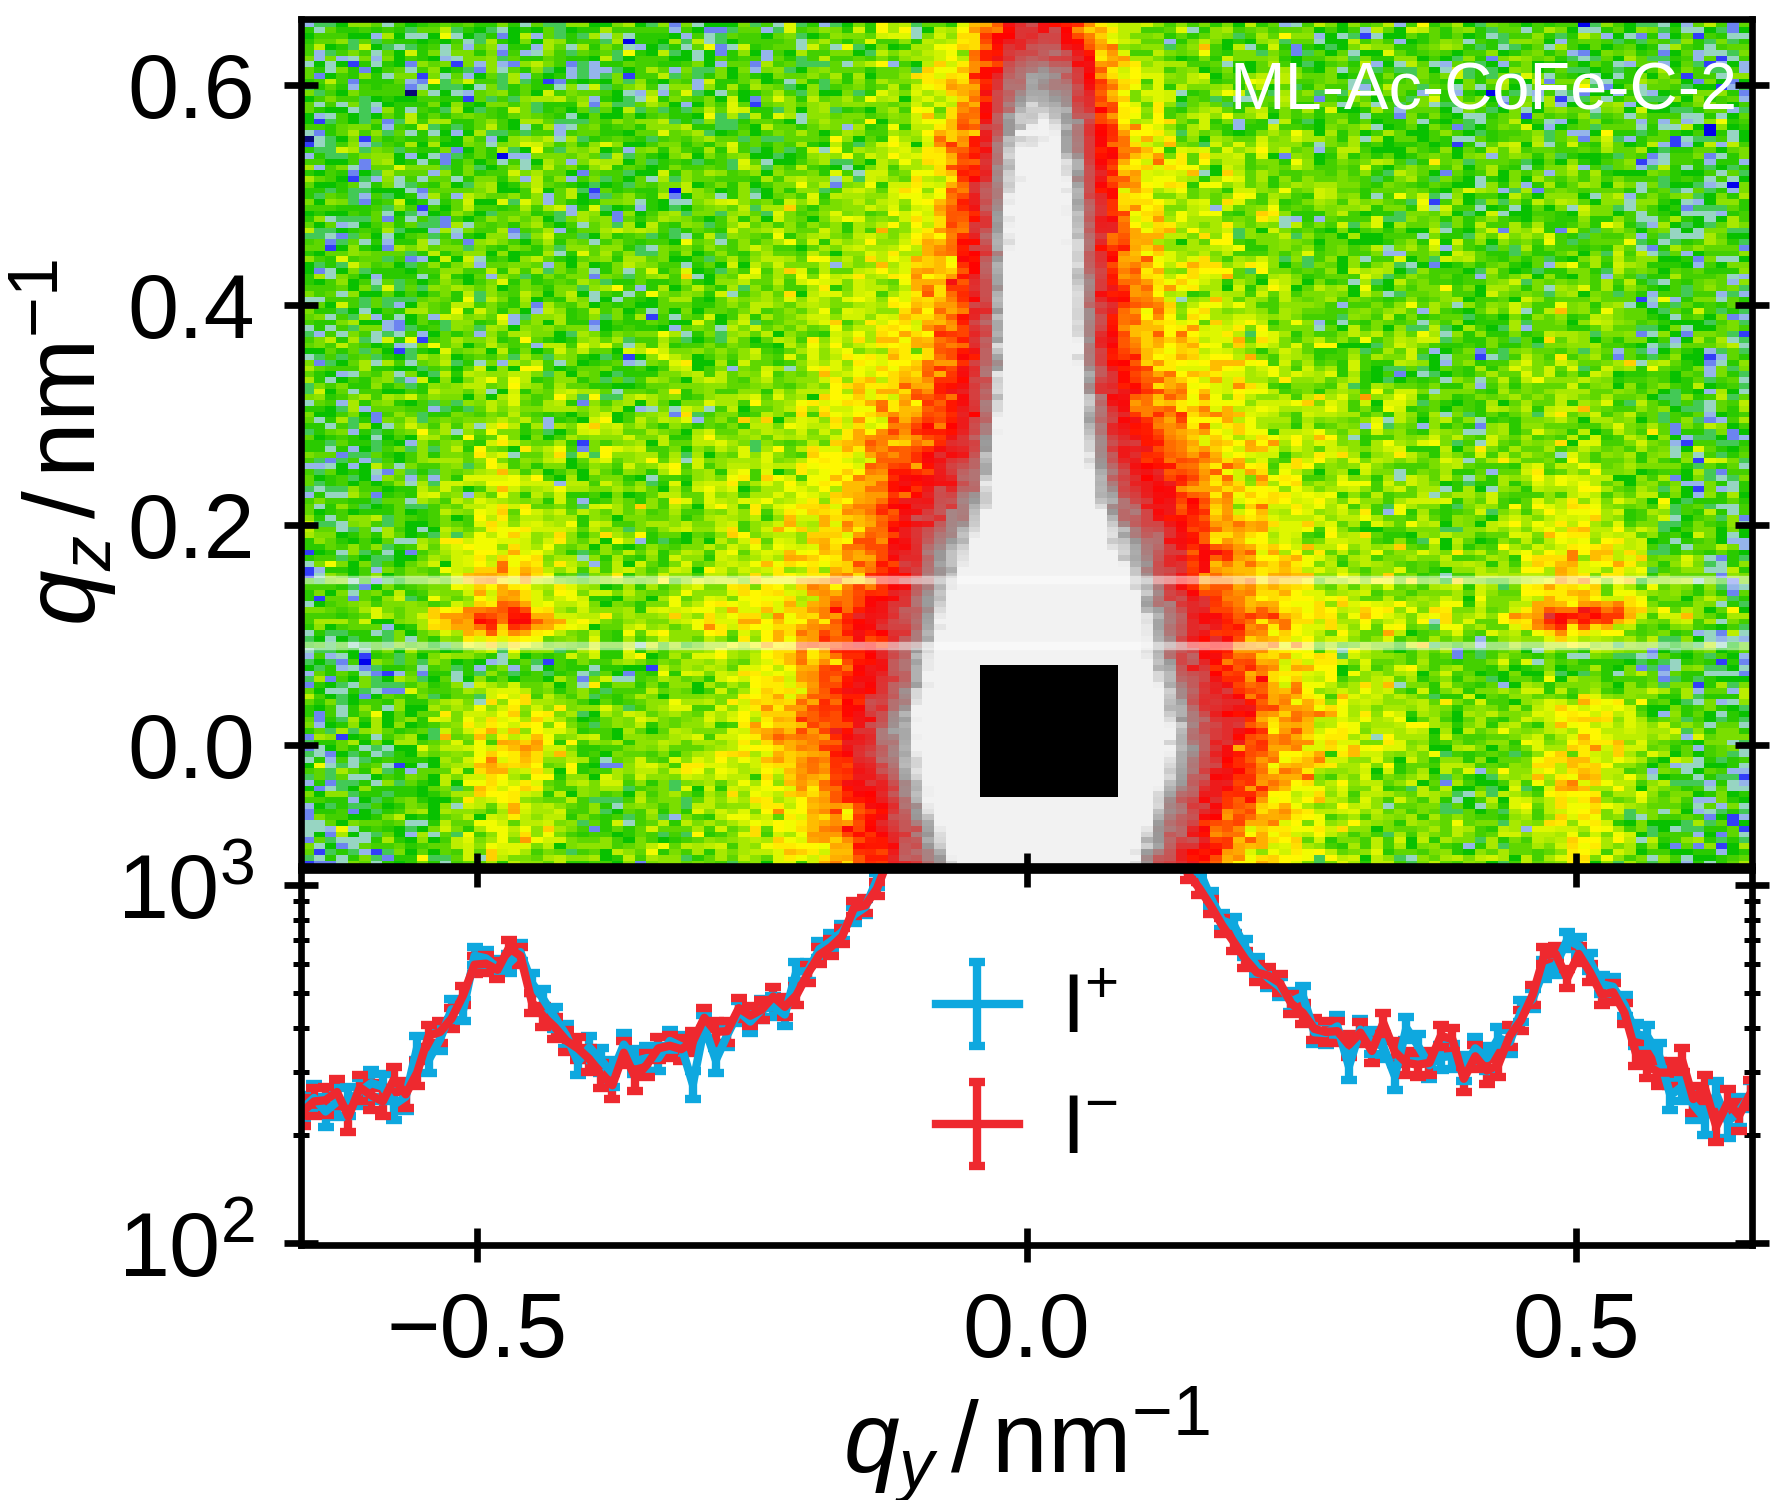
\includegraphics{monolayers_GISANS_ML-Ac-CoFe-C-2_ZFC5K_GF}
    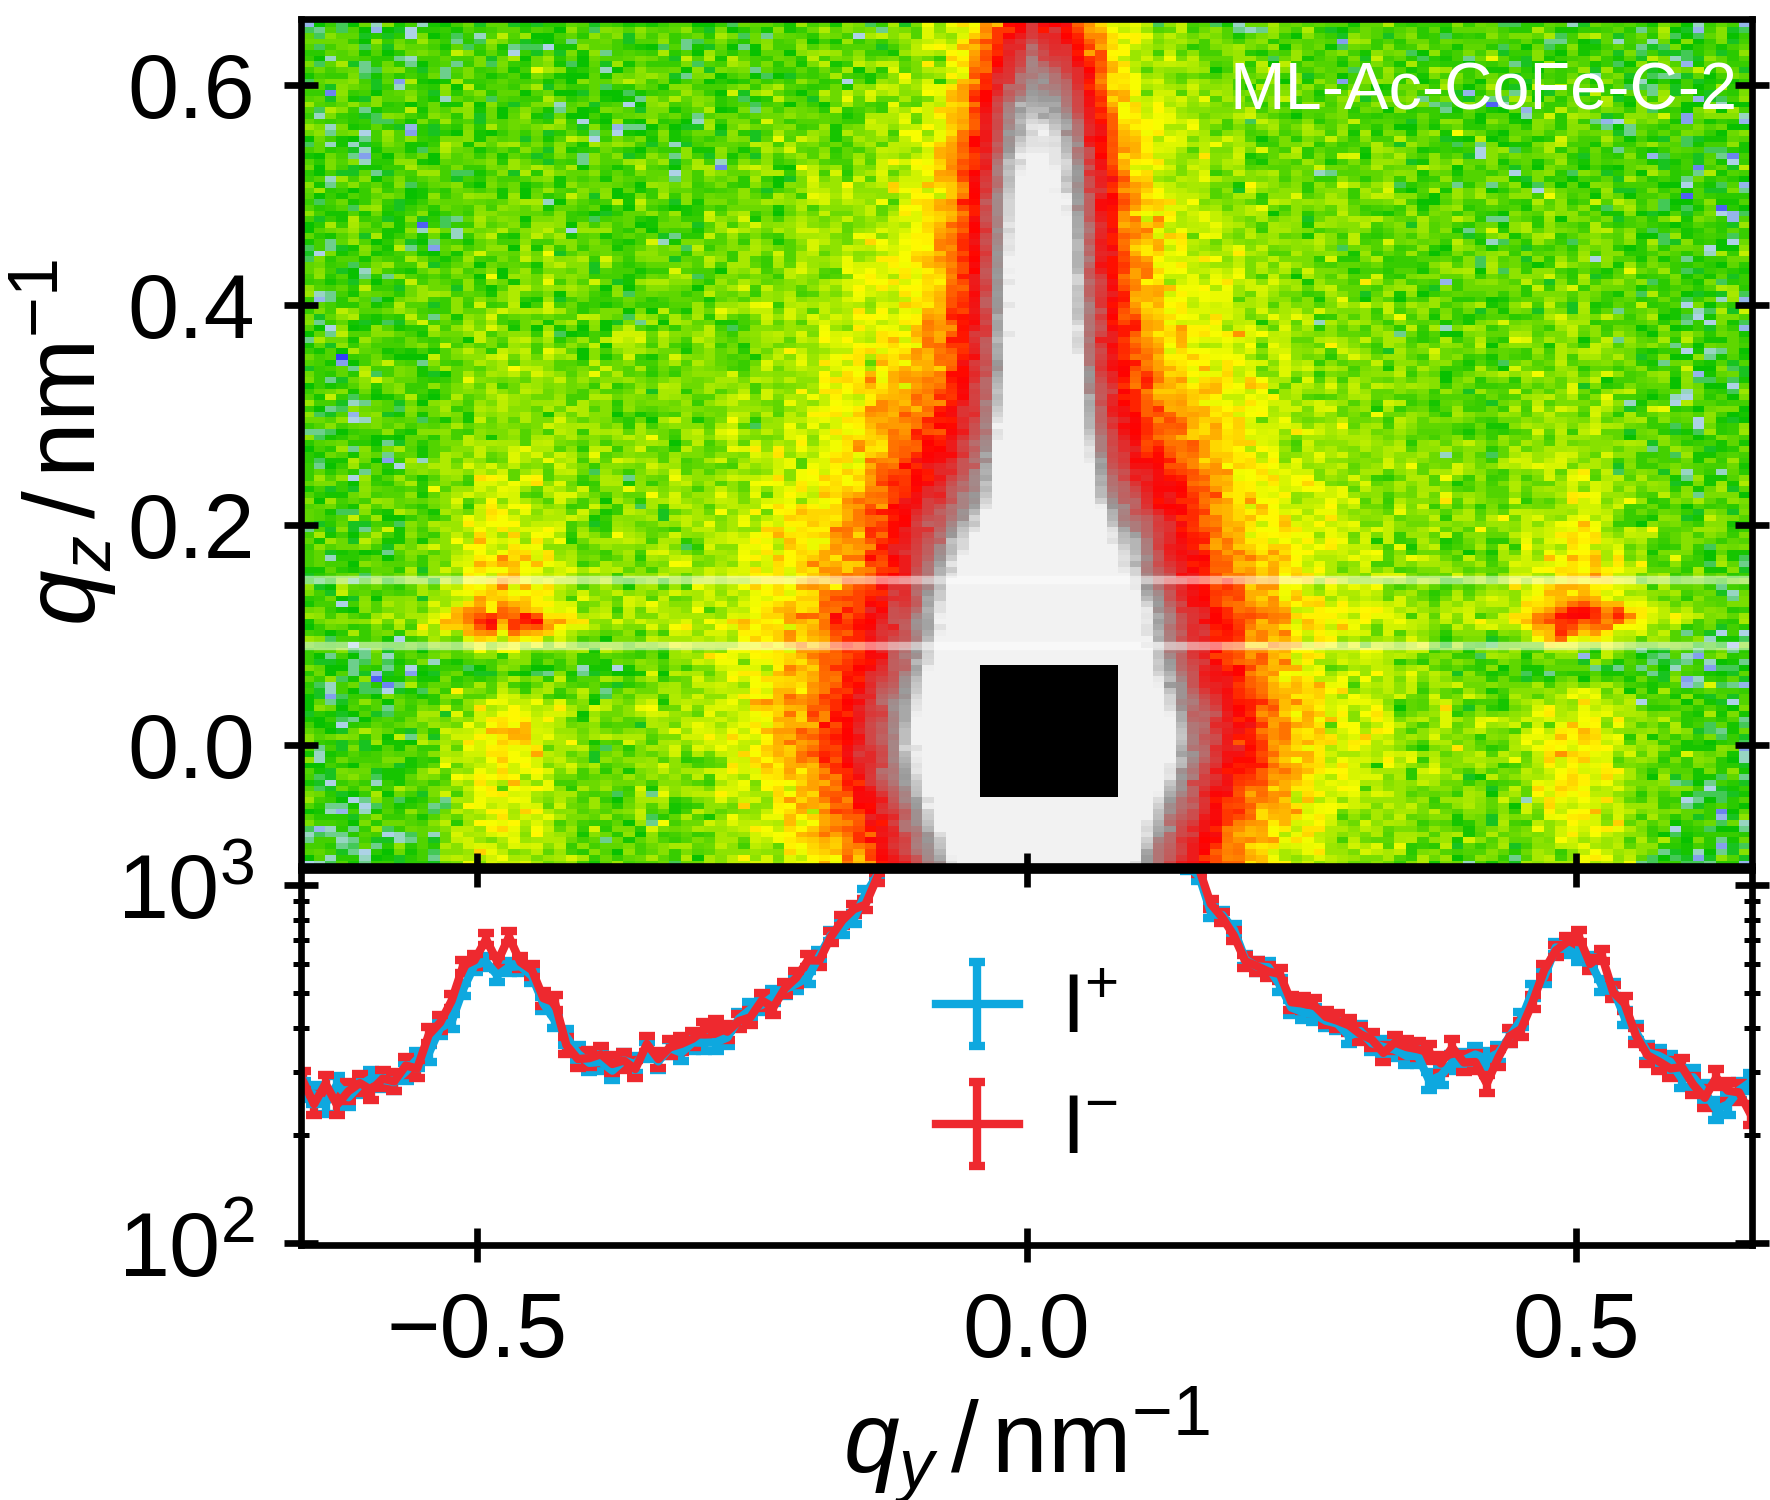
\includegraphics{monolayers_GISANS_ML-Ac-CoFe-C-2_ZFC5K_Remanence}
    \caption{\label{fig:monolayer:magneticStructure:polGisans5KZFC}Polarized grazing-incidence small-angle neutron scattering of ML-Ac-CoFe-C-2 after zero-field cooling to $5 \unit{K}$. Left is the detector image $I^{+}$ measured at guide field ($5 \unit{mT}$) after zero-field cooling and right the detector image of $I^{+}$ in remanence after exposing the sample to a field of $4 \unit{T}$ parallel to the neutron beam and subsequently turning back to guide field. The lower plots show the projection of the Yoneda band for both $I^{+}$ and $I^{-}$ and the nuclear peak position and half it's value are marked by black lines.}
  \end{figure}
  Polarized GISANS is used to discuss whether a macroscopic super antiferromagnetic state is present in the sample ML-Ac-CoFe-C-2, which consists of nanocubes ordered in a square array.
  As a technique to resolve lateral correlations in a nanostructure that is also sensitive to the magnetic structure, GISANS is ideal for this purpose as it is expected that a super antiferromagnetic structure shows additionally to the nuclear scattering peaks with the period of the lattice, magnetic scattering with the double period.
  Due to symmetry this effect should also be independent of the neutron polarization and therefore visible in both channels $I^{+}$ and $I^{-}$.
  \reffig{fig:monolayer:magneticStructure:polGisans5KZFC} shows the polarized GISANS images ($I^{+}$) measured at D33 for ML-Ac-CoFe-C-2 after zero-field cooling to $5 \unit{K}$ measured in in the initial state and at remanence after the application of a $4 \unit{T}$ field parallel to the beam with a guide field of $5 \unit{mT}$ in both cases.

  In the Yoneda band, the first order nuclear peak is clearly visible in both cases around $0.5 \unit{nm^{-1}}$.
  Within the counting error, no significant difference is visible between the two polarization channels.
  From the nuclear peak position, the expected position for the super antiferromagnetic peak at the double period is marked, where however no significant peak is visible.

  \begin{figure}[tb]
    \centering
    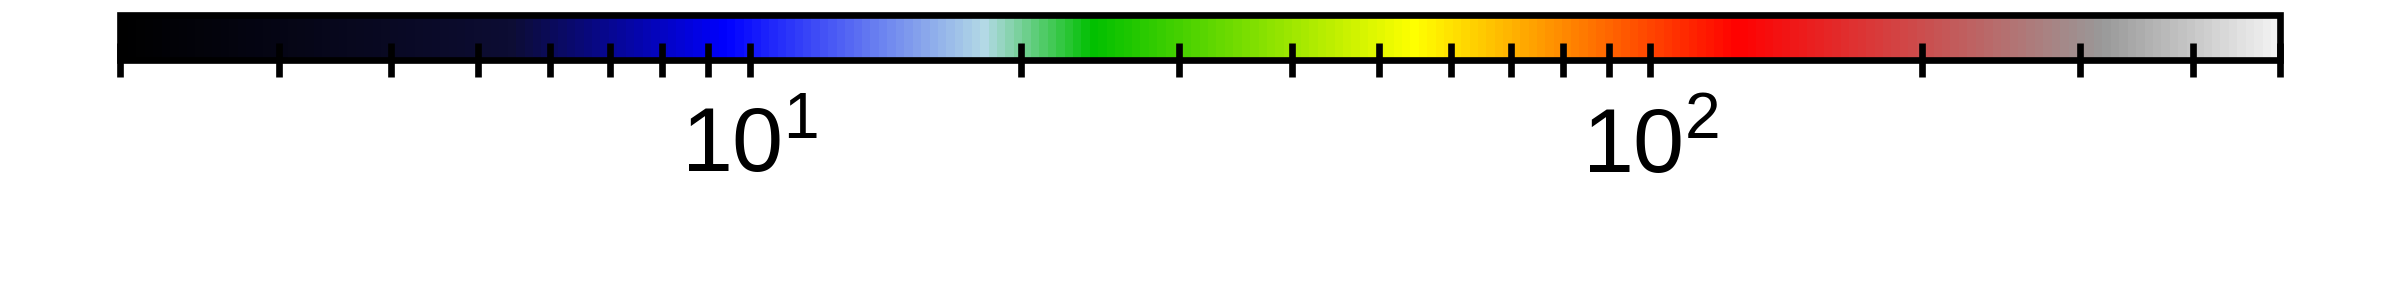
\includegraphics{monolayers_ML-Ac-CoFe-C_GISANS_SVcbar_perpendicularBeam}
    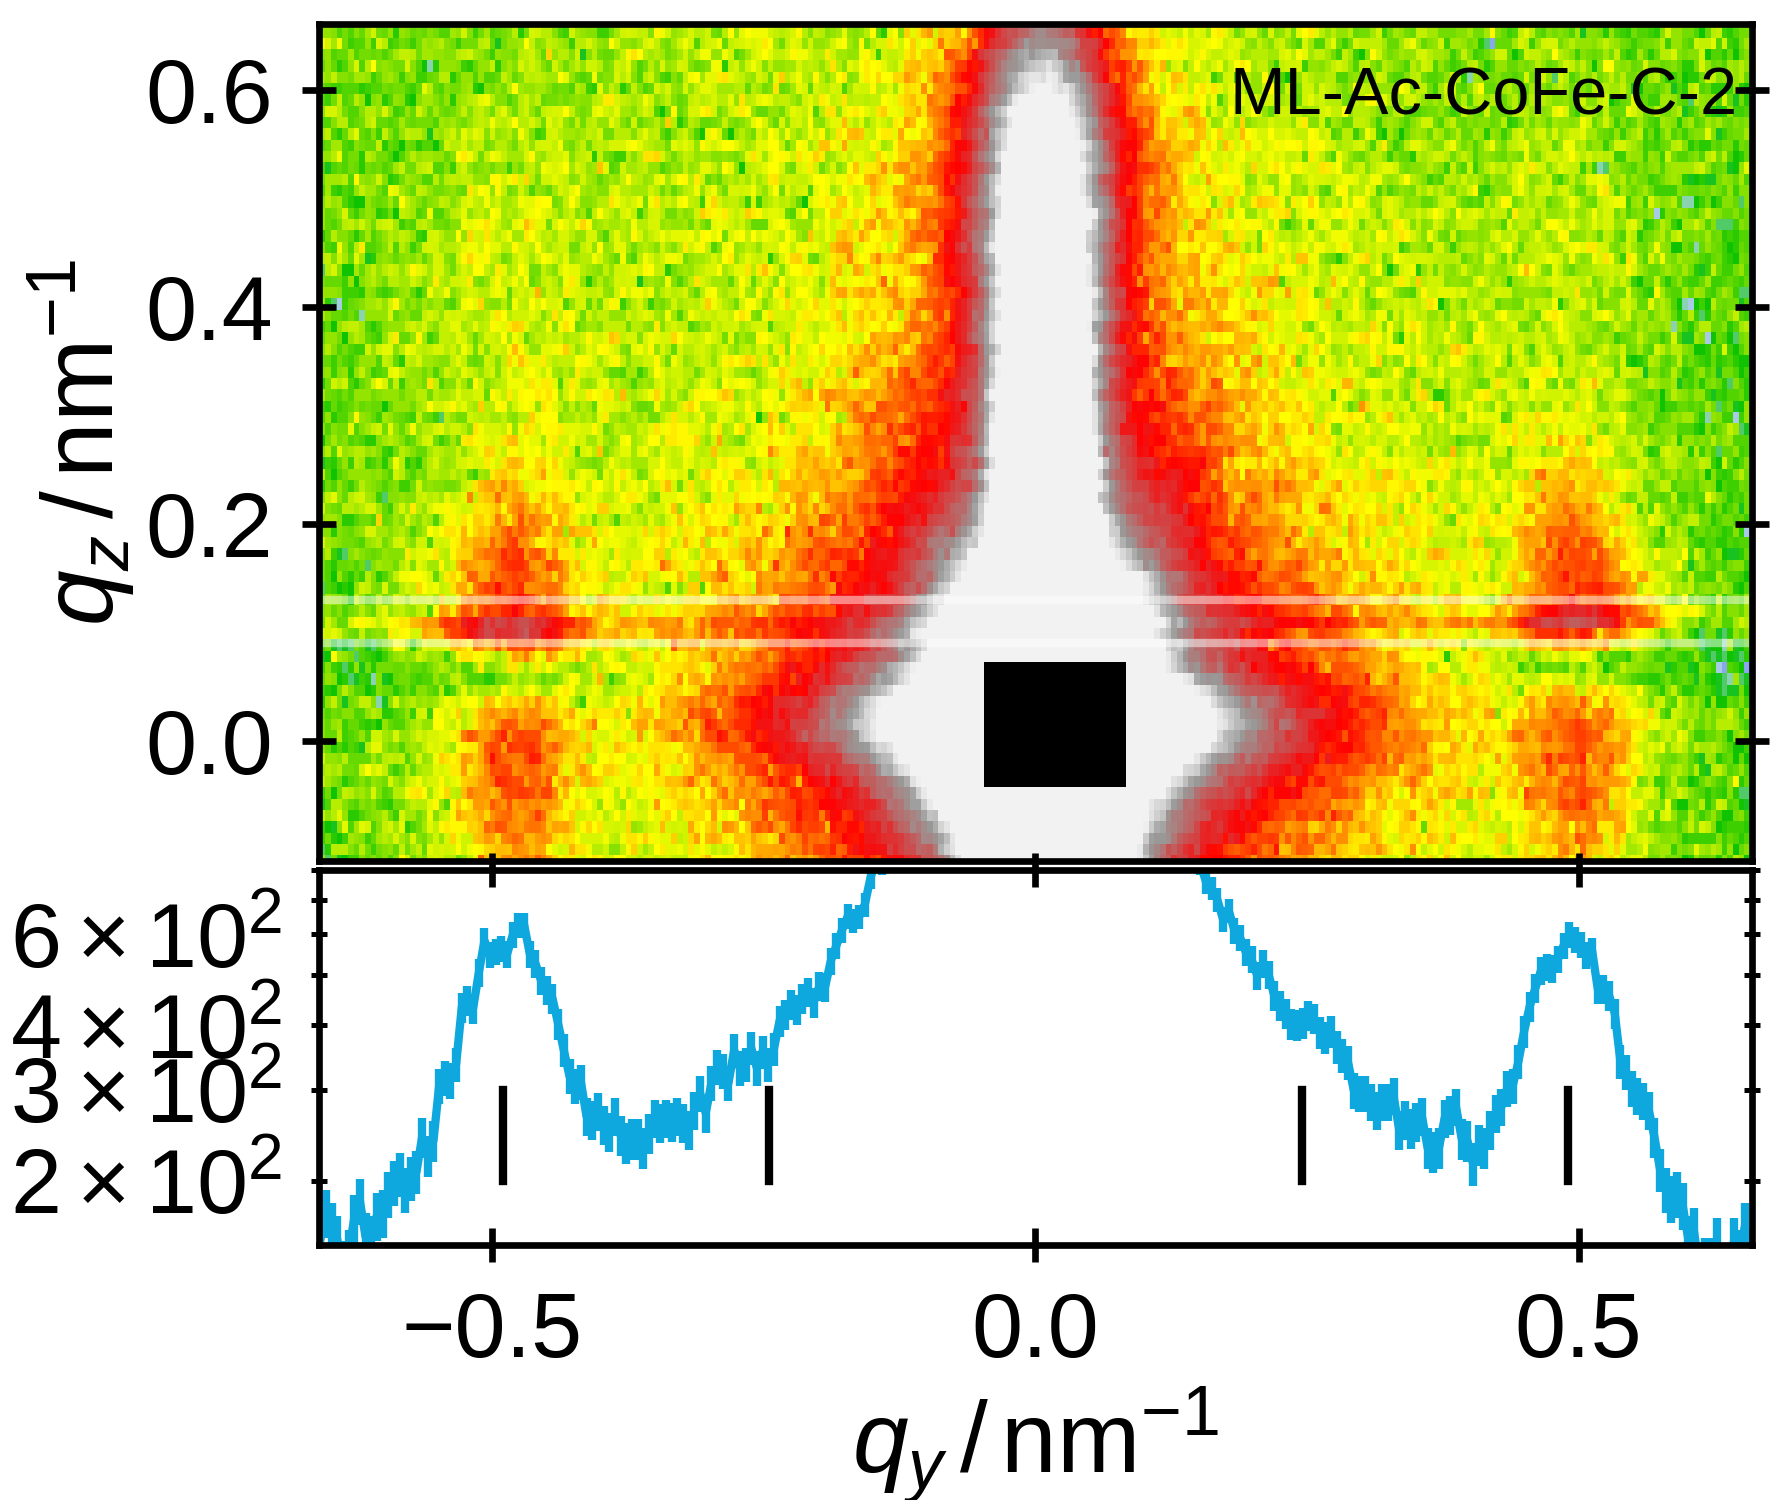
\includegraphics{monolayers_GISANS_ML-Ac-CoFe-C-2_ZFC5K_Unpolarized_GF}
    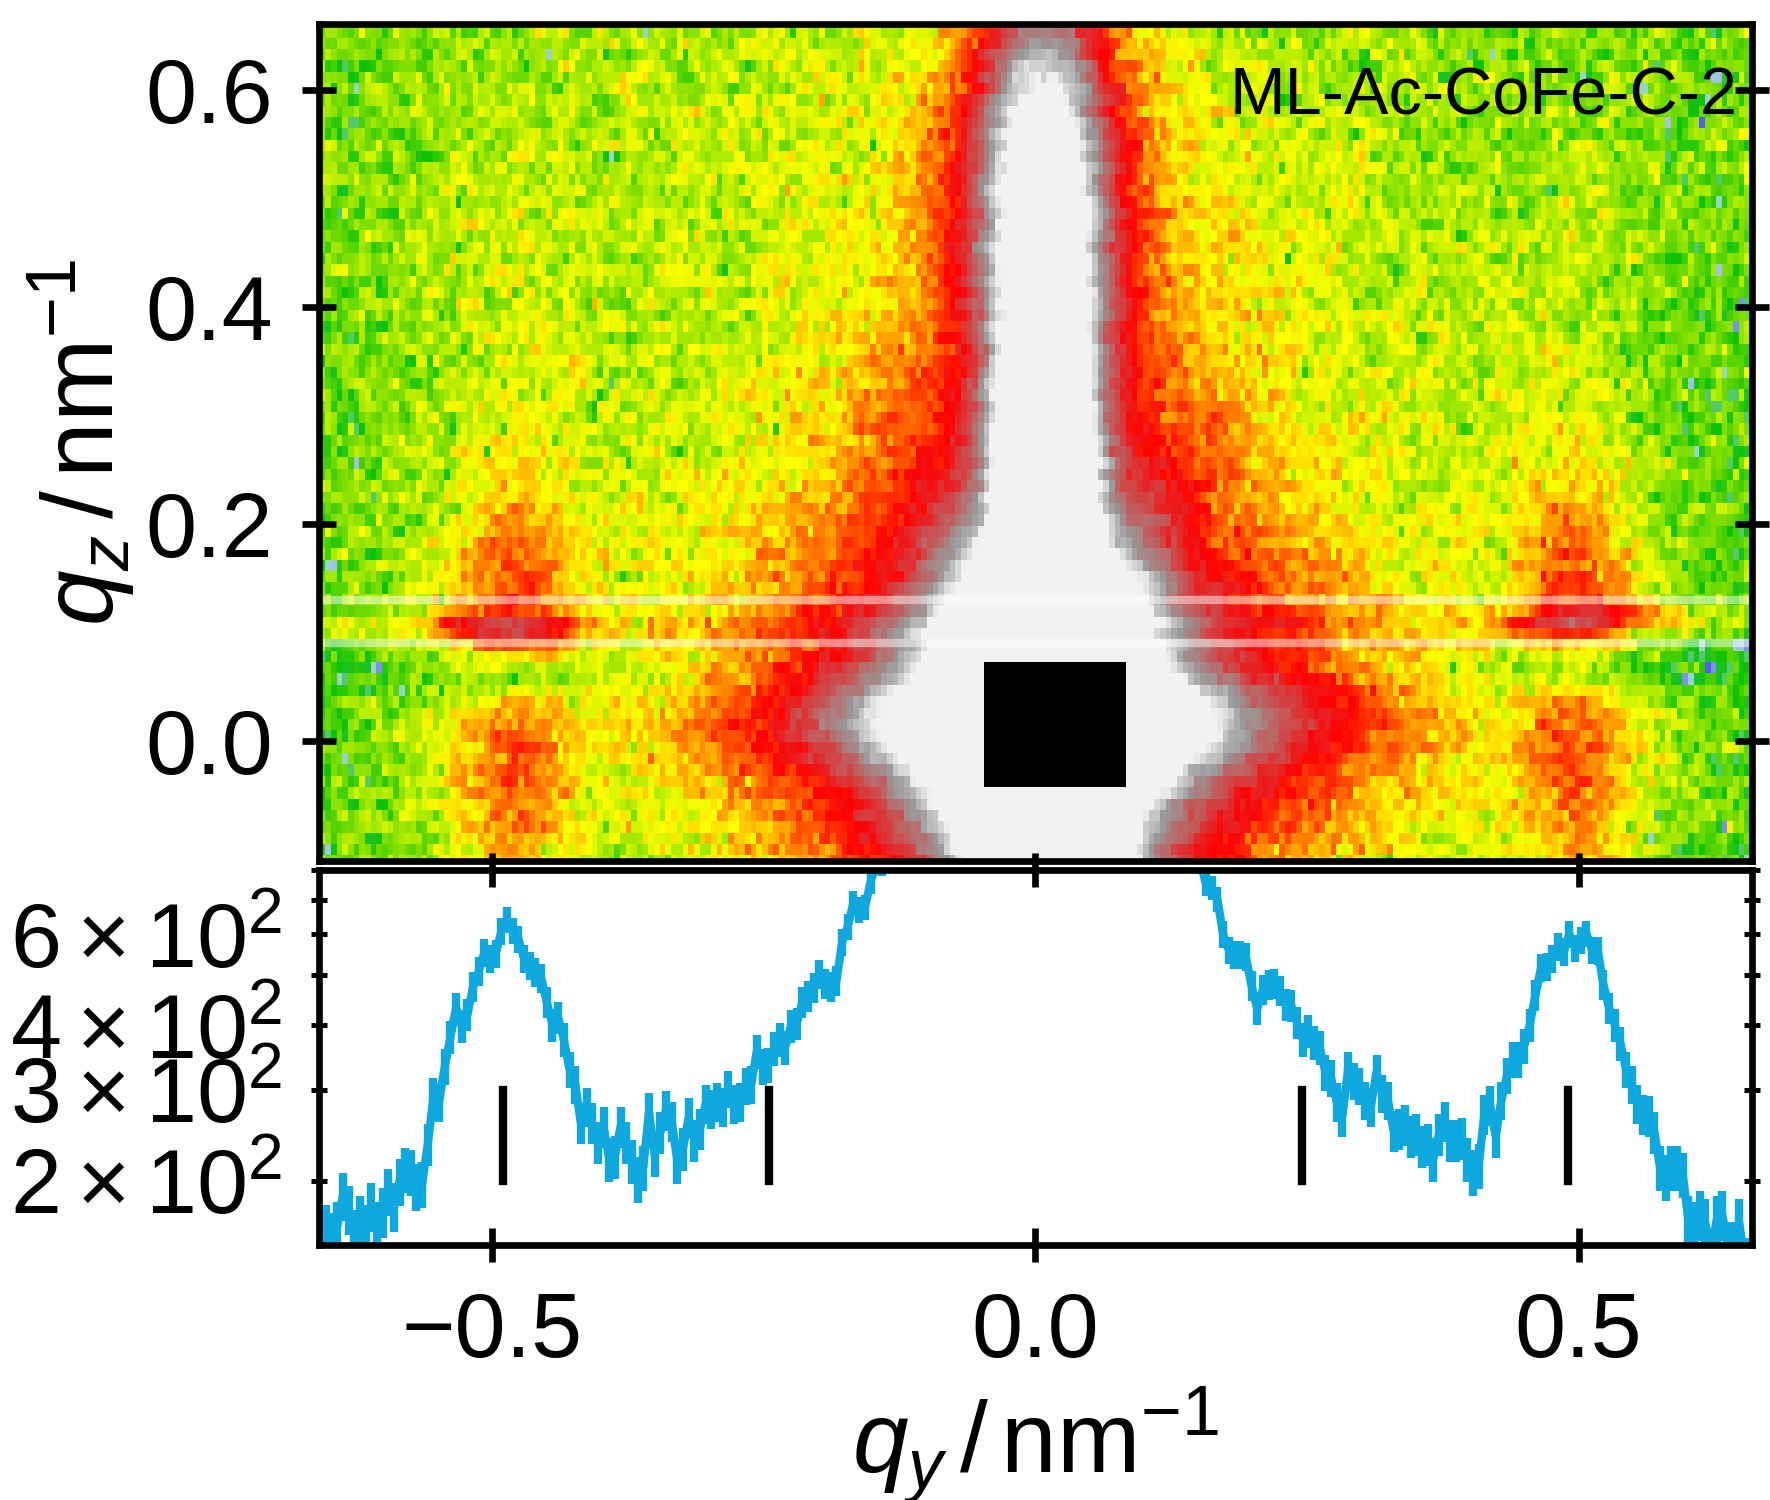
\includegraphics{monolayers_GISANS_ML-Ac-CoFe-C-2_ZFC5K_Unpolarized_Remanence}
    \caption{\label{fig:monolayer:magneticStructure:Gisans5KZFCperpendicular}GISANS of ML-Ac-CoFe-C-2 after zero-field cooling to $5 \unit{K}$. The sample is measured initially at the guide field of $5 \unit{mT}$ (left) and in remanence after application of a $4 \unit{T}$ field in the sample plane, perpendicular to the neutron beam. The lower plots show the projection of the Yoneda band.}
  \end{figure}

  In \reffig{fig:monolayer:magneticStructure:Gisans5KZFCperpendicular}, the same measurement, without distinction of the incoming neutron polarization, is performed but with the $4 \unit{T}$ field applied perpendicular to the beam in the sample plane.
  The counting statistics is slightly improved as both neutron channels are measured simultaneously.
  With good will, a slight increase in intensity is visible in the measurements around the expected region for the super antiferromagnetic peak at $q_y \eq 0.25 \unit{nm^{-1}}$, but it could also be considered a statistical fluctuation as it is not symmetrically visible in the negative $q_y$ range.
  
  Additional measurements performed at $250 \unit{K}$ with the applied field parallel and perpendicular to the beam in the sample plane show no different results (not shown) and thus it can be concluded that if any super antiferromagnetic peak is present in the sample, it is heavily smeared out and hidden in the background.

  
  \begin{figure}[tb]
    \centering
    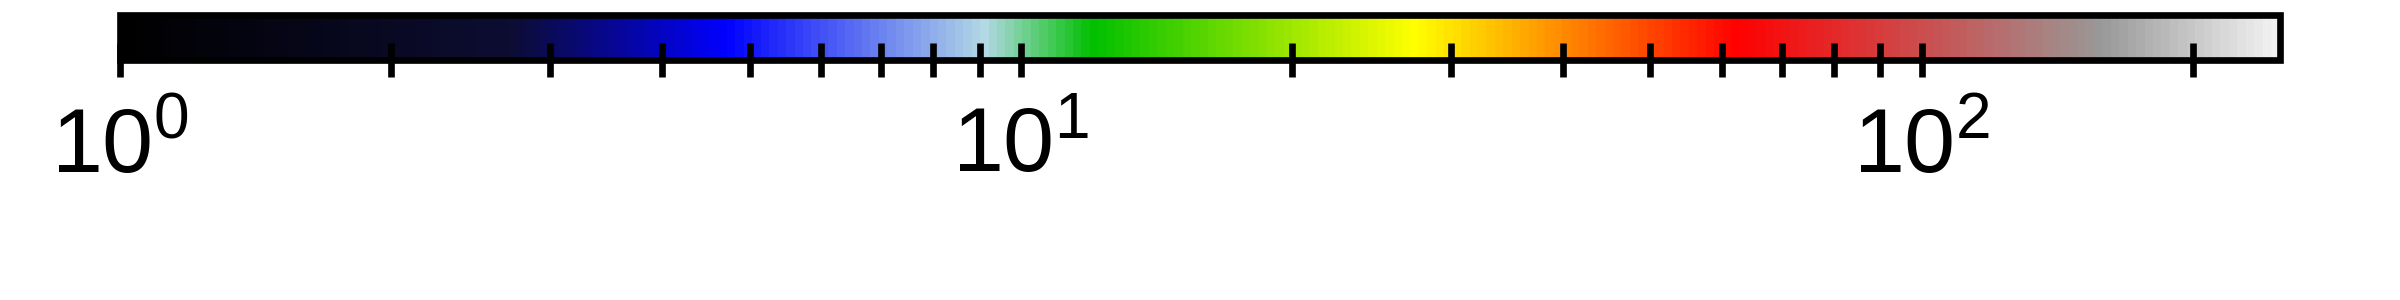
\includegraphics{monolayers_ML-Ac-CoFe-C_GISANS_SVcbar_negField}
    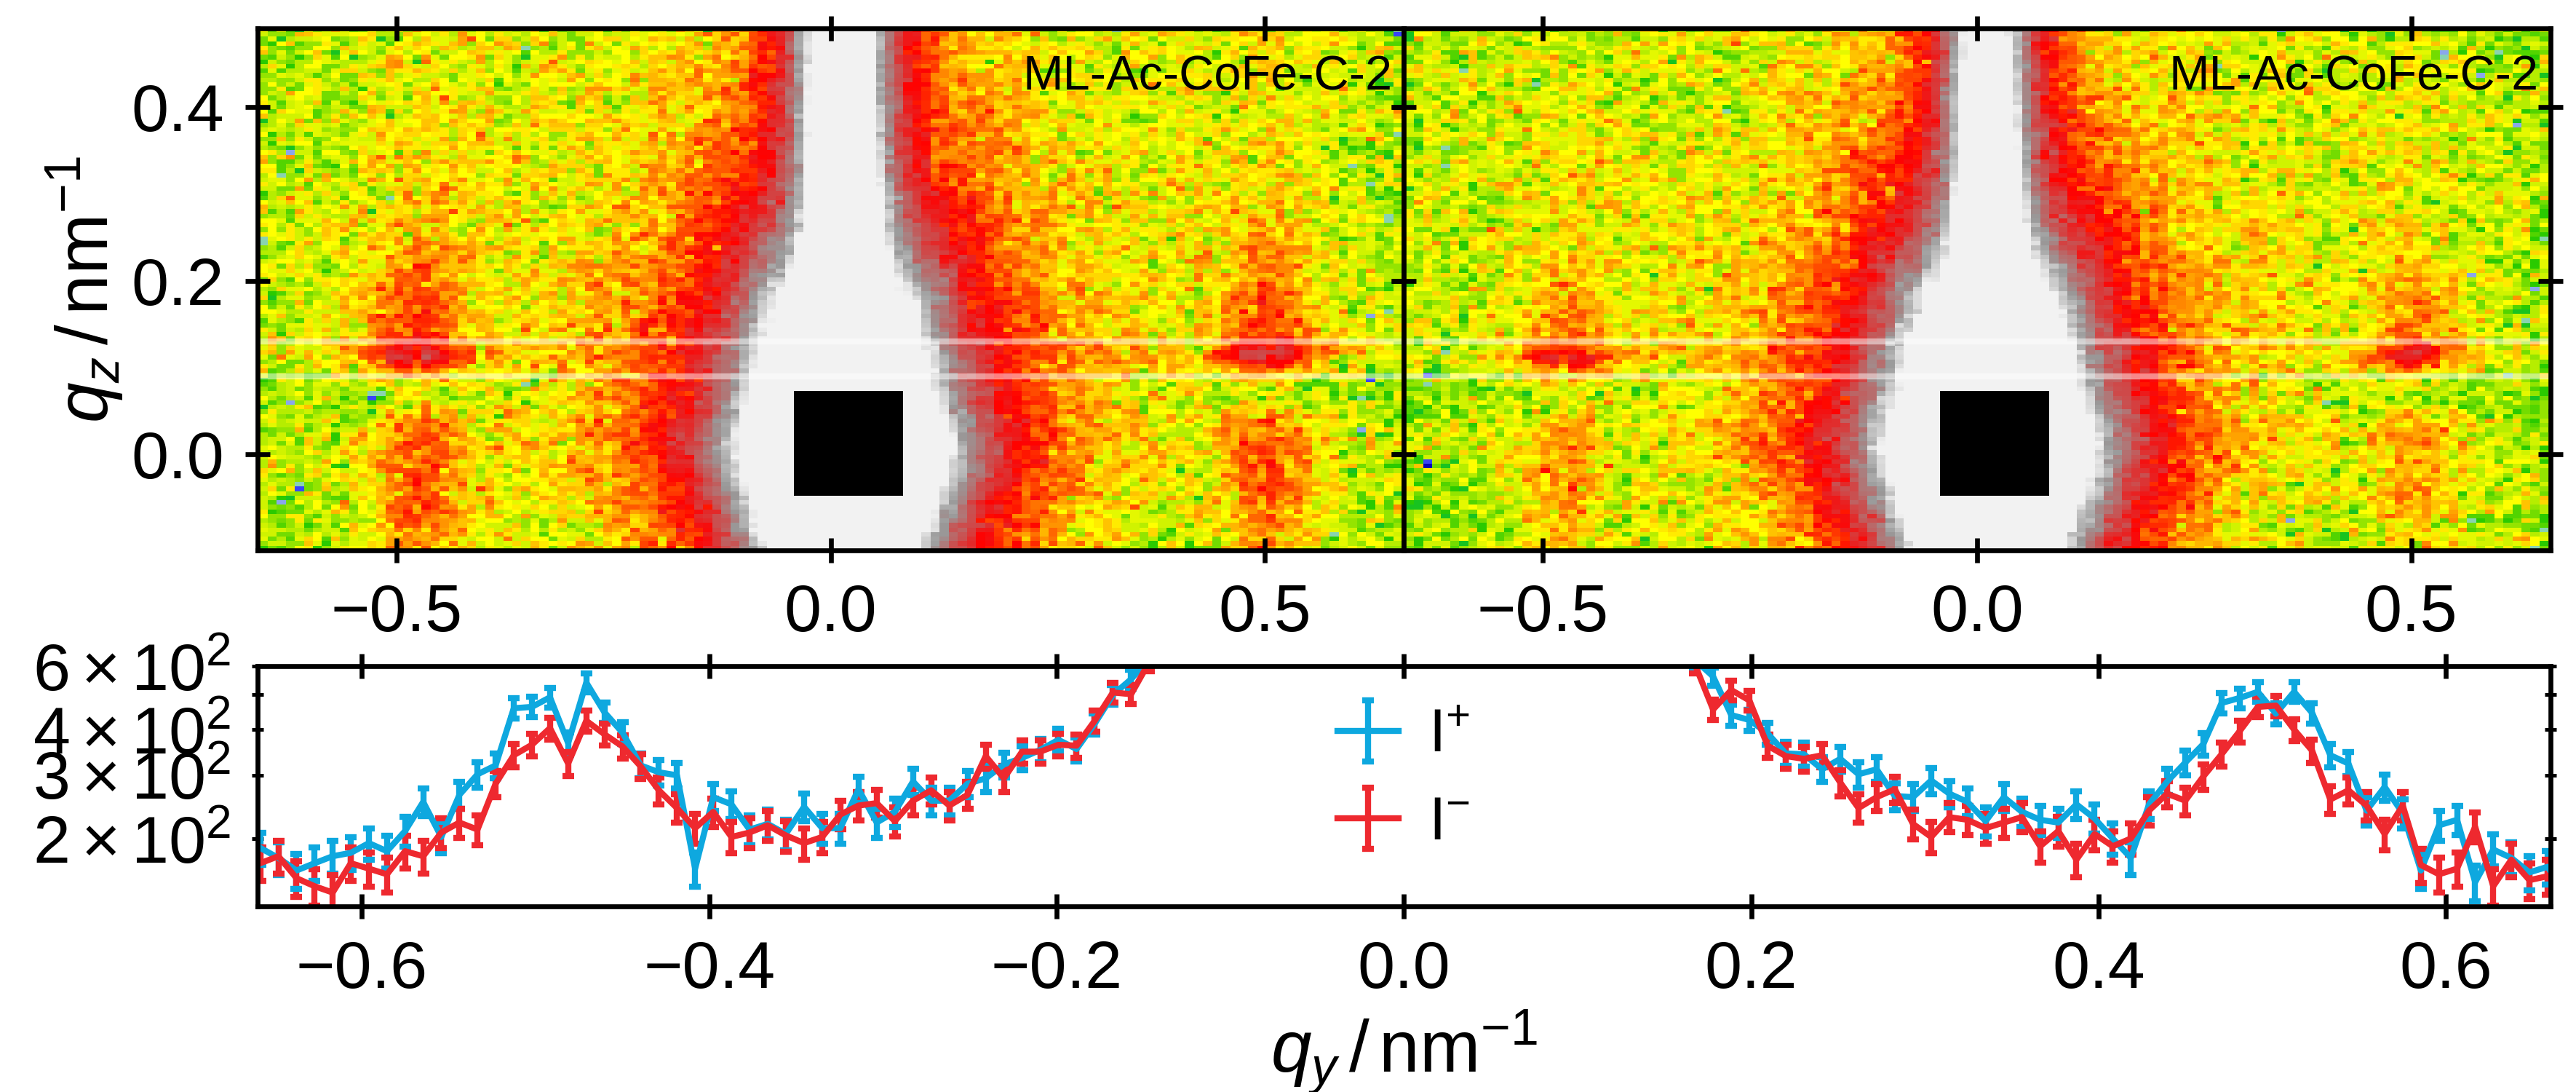
\includegraphics{monolayers_GISANS_ML-Ac-CoFe-C-2_ZFC5K_negField}
    \caption{\label{fig:monolayer:magneticStructure:negativeField}PolGISANS of ML-Ac-CoFe-C-2 after ZFC and saturation in a magnetic field of $4 \unit{T}$ analogue to \reffig{fig:monolayer:magneticStructure:polGisans5KZFC} measured in a negative magnetic field $-200 \unit{mT}$ applied parallel to the neutron beam. The left detector image shows $I^{+}$ and the right image $I^{-}$. The lower plot shows the Yoneda band of both detector images.}
  \end{figure}

  Another attempt was performed in measuring the polGISANS at a negative field of $-200 \unit{mT}$ parallel to the neutron beam after the zero-field cooling procedure and saturation at $4 \unit{T}$, which is shown in \reffig{fig:monolayer:magneticStructure:negativeField}.
  A magnetic contrast is visible in both the detector images and the Yoneda band.
  It is noteworthy, that this splitting is observed in the case of a negatively applied field but not for the previously discussed remanent case.
  With $I^{+} > I^{-}$ at a negative magnetic field it can be concluded, that the magnetization of the sample is preferentially parallel to the neutron beam direction.

\end{document}